\PassOptionsToPackage{unicode=true}{hyperref} % options for packages loaded elsewhere
\PassOptionsToPackage{hyphens}{url}
%
\documentclass[
  10pt,
  ignorenonframetext,
]{beamer}
\usepackage{pgfpages}
\setbeamertemplate{caption}[numbered]
\setbeamertemplate{caption label separator}{: }
\setbeamercolor{caption name}{fg=normal text.fg}
\beamertemplatenavigationsymbolsempty
% Prevent slide breaks in the middle of a paragraph:
\widowpenalties 1 10000
\raggedbottom
\setbeamertemplate{part page}{
  \centering
  \begin{beamercolorbox}[sep=16pt,center]{part title}
    \usebeamerfont{part title}\insertpart\par
  \end{beamercolorbox}
}
\setbeamertemplate{section page}{
  \centering
  \begin{beamercolorbox}[sep=12pt,center]{part title}
    \usebeamerfont{section title}\insertsection\par
  \end{beamercolorbox}
}
\setbeamertemplate{subsection page}{
  \centering
  \begin{beamercolorbox}[sep=8pt,center]{part title}
    \usebeamerfont{subsection title}\insertsubsection\par
  \end{beamercolorbox}
}
\AtBeginPart{
  \frame{\partpage}
}
\AtBeginSection{
  \ifbibliography
  \else
    \frame{\sectionpage}
  \fi
}
\AtBeginSubsection{
  \frame{\subsectionpage}
}
\usepackage{lmodern}
\usepackage{amssymb,amsmath}
\usepackage{ifxetex,ifluatex}
\ifnum 0\ifxetex 1\fi\ifluatex 1\fi=0 % if pdftex
  \usepackage[T1]{fontenc}
  \usepackage[utf8]{inputenc}
  \usepackage{textcomp} % provides euro and other symbols
\else % if luatex or xelatex
  \usepackage{unicode-math}
  \defaultfontfeatures{Scale=MatchLowercase}
  \defaultfontfeatures[\rmfamily]{Ligatures=TeX,Scale=1}
\fi
\usetheme[]{Dresden}
\usecolortheme{dolphin}
\usefonttheme{structuresmallcapsserif}
% use upquote if available, for straight quotes in verbatim environments
\IfFileExists{upquote.sty}{\usepackage{upquote}}{}
\IfFileExists{microtype.sty}{% use microtype if available
  \usepackage[]{microtype}
  \UseMicrotypeSet[protrusion]{basicmath} % disable protrusion for tt fonts
}{}
\makeatletter
\@ifundefined{KOMAClassName}{% if non-KOMA class
  \IfFileExists{parskip.sty}{%
    \usepackage{parskip}
  }{% else
    \setlength{\parindent}{0pt}
    \setlength{\parskip}{6pt plus 2pt minus 1pt}}
}{% if KOMA class
  \KOMAoptions{parskip=half}}
\makeatother
\usepackage{xcolor}
\IfFileExists{xurl.sty}{\usepackage{xurl}}{} % add URL line breaks if available
\IfFileExists{bookmark.sty}{\usepackage{bookmark}}{\usepackage{hyperref}}
\hypersetup{
  pdftitle={Supervised Learning - Regression Trees and Bagging},
  pdfauthor={Jan-Philipp Kolb},
  pdfborder={0 0 0},
  breaklinks=true}
\urlstyle{same}  % don't use monospace font for urls
\newif\ifbibliography
\usepackage{color}
\usepackage{fancyvrb}
\newcommand{\VerbBar}{|}
\newcommand{\VERB}{\Verb[commandchars=\\\{\}]}
\DefineVerbatimEnvironment{Highlighting}{Verbatim}{commandchars=\\\{\}}
% Add ',fontsize=\small' for more characters per line
\newenvironment{Shaded}{}{}
\newcommand{\AlertTok}[1]{\textcolor[rgb]{1.00,0.00,0.00}{#1}}
\newcommand{\AnnotationTok}[1]{\textcolor[rgb]{0.00,0.50,0.00}{#1}}
\newcommand{\AttributeTok}[1]{#1}
\newcommand{\BaseNTok}[1]{#1}
\newcommand{\BuiltInTok}[1]{#1}
\newcommand{\CharTok}[1]{\textcolor[rgb]{0.00,0.50,0.50}{#1}}
\newcommand{\CommentTok}[1]{\textcolor[rgb]{0.00,0.50,0.00}{#1}}
\newcommand{\CommentVarTok}[1]{\textcolor[rgb]{0.00,0.50,0.00}{#1}}
\newcommand{\ConstantTok}[1]{#1}
\newcommand{\ControlFlowTok}[1]{\textcolor[rgb]{0.00,0.00,1.00}{#1}}
\newcommand{\DataTypeTok}[1]{#1}
\newcommand{\DecValTok}[1]{#1}
\newcommand{\DocumentationTok}[1]{\textcolor[rgb]{0.00,0.50,0.00}{#1}}
\newcommand{\ErrorTok}[1]{\textcolor[rgb]{1.00,0.00,0.00}{\textbf{#1}}}
\newcommand{\ExtensionTok}[1]{#1}
\newcommand{\FloatTok}[1]{#1}
\newcommand{\FunctionTok}[1]{#1}
\newcommand{\ImportTok}[1]{#1}
\newcommand{\InformationTok}[1]{\textcolor[rgb]{0.00,0.50,0.00}{#1}}
\newcommand{\KeywordTok}[1]{\textcolor[rgb]{0.00,0.00,1.00}{#1}}
\newcommand{\NormalTok}[1]{#1}
\newcommand{\OperatorTok}[1]{#1}
\newcommand{\OtherTok}[1]{\textcolor[rgb]{1.00,0.25,0.00}{#1}}
\newcommand{\PreprocessorTok}[1]{\textcolor[rgb]{1.00,0.25,0.00}{#1}}
\newcommand{\RegionMarkerTok}[1]{#1}
\newcommand{\SpecialCharTok}[1]{\textcolor[rgb]{0.00,0.50,0.50}{#1}}
\newcommand{\SpecialStringTok}[1]{\textcolor[rgb]{0.00,0.50,0.50}{#1}}
\newcommand{\StringTok}[1]{\textcolor[rgb]{0.00,0.50,0.50}{#1}}
\newcommand{\VariableTok}[1]{#1}
\newcommand{\VerbatimStringTok}[1]{\textcolor[rgb]{0.00,0.50,0.50}{#1}}
\newcommand{\WarningTok}[1]{\textcolor[rgb]{0.00,0.50,0.00}{\textbf{#1}}}
\usepackage{graphicx,grffile}
\makeatletter
\def\maxwidth{\ifdim\Gin@nat@width>\linewidth\linewidth\else\Gin@nat@width\fi}
\def\maxheight{\ifdim\Gin@nat@height>\textheight\textheight\else\Gin@nat@height\fi}
\makeatother
% Scale images if necessary, so that they will not overflow the page
% margins by default, and it is still possible to overwrite the defaults
% using explicit options in \includegraphics[width, height, ...]{}
\setkeys{Gin}{width=\maxwidth,height=\maxheight,keepaspectratio}
\setlength{\emergencystretch}{3em}  % prevent overfull lines
\providecommand{\tightlist}{%
  \setlength{\itemsep}{0pt}\setlength{\parskip}{0pt}}
\setcounter{secnumdepth}{-2}

% set default figure placement to htbp
\makeatletter
\def\fps@figure{htbp}
\makeatother


\title{Supervised Learning - Regression Trees and Bagging}
\author{Jan-Philipp Kolb}
\date{04 Juni, 2019}

\begin{document}
\frame{\titlepage}

\begin{frame}{\href{https://www.statmethods.net/advstats/cart.html}{Tree-Based
Models}}
\protect\hypertarget{tree-based-models}{}

\begin{itemize}
\item
  Trees are good for interpretation because they are simple
\item
  Tree based methods involve stratifying or segmenting the predictor
  space into a number of simple regions.
  (\href{https://lagunita.stanford.edu/c4x/HumanitiesScience/StatLearning/asset/trees.pdf}{\textbf{Hastie
  and Tibshirani}})
\end{itemize}

\begin{block}{But:}

\begin{itemize}
\tightlist
\item
  These methods do not deliver the best results concerning prediction
  accuracy.
\end{itemize}

\end{block}

\begin{block}{Source of slides}

\begin{itemize}
\tightlist
\item
  The following slides are based on the UC Business Analytics R
  Programming Guide on
  \href{http://uc-r.github.io/regression_trees}{\textbf{regression
  trees}}
\end{itemize}

\end{block}

\end{frame}

\begin{frame}{The Idea}
\protect\hypertarget{the-idea}{}

\begin{itemize}
\tightlist
\item
  There are many methodologies for constructing regression trees but one
  of the oldest is the
  \href{https://machinelearningmastery.com/classification-and-regression-trees-for-machine-learning/}{\textbf{classification
  and regression tree}} (CART) approach by Breiman et al.~(1984).
\item
  Basic
  \href{https://towardsdatascience.com/the-complete-guide-to-decision-trees-28a4e3c7be14}{\textbf{regression
  trees partition a data set into smaller subgroups}} and then fit a
  simple constant for each observation in the subgroup.
\item
  The partitioning is achieved by successive
  \href{https://en.wikipedia.org/wiki/Binary_space_partitioning}{\textbf{binary
  partitions}} (aka
  \href{https://en.wikipedia.org/wiki/Recursive_partitioning}{recursive
  partitioning}) based on the different predictors.
\item
  The constant to predict is based on the average response values for
  all observations that fall in that subgroup.
\end{itemize}

\end{frame}

\begin{frame}{Explanation:
\href{https://en.wikipedia.org/wiki/Decision_tree}{\textbf{decision
tree}}}
\protect\hypertarget{explanation-decision-tree}{}

Decision trees model data as a ``tree'' of hierarchical branches. They
make branches until they reach ``leaves'' that represent predictions.

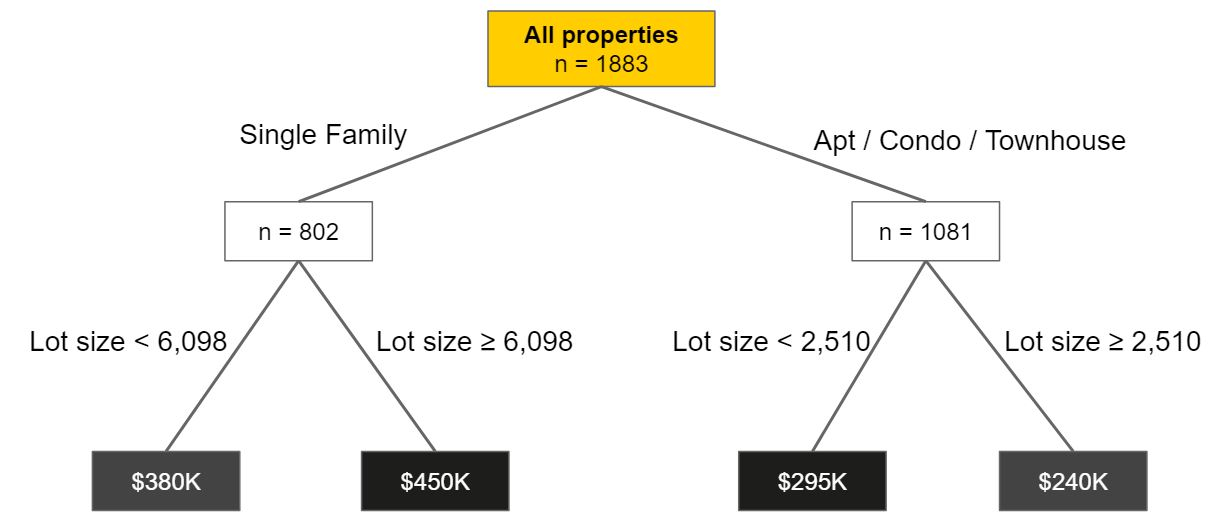
\includegraphics{figure/Decision-Tree-Example.jpg}

\end{frame}

\begin{frame}{Example decission trees}
\protect\hypertarget{example-decission-trees}{}

Due to their branching structure, decision trees can easily model
nonlinear relationships.

\begin{block}{Example}

\begin{itemize}
\tightlist
\item
  For single family homes (larger lots) higher prices,
\item
  and for apartments (smaller lots), also higher prices (because here
  it's a proxy for urban / rural).
\end{itemize}

This reversal of correlation is difficult for linear models to capture
unless you explicitly add an interaction term

\begin{itemize}
\tightlist
\item
  Decision trees can capture this relationship naturally.
\end{itemize}

\end{block}

\end{frame}

\begin{frame}{Model foundations}
\protect\hypertarget{model-foundations}{}

\begin{itemize}
\tightlist
\item
  This simple example can be generalized
\item
  We have a continuous response variable \(Y\) and two inputs \(X_1\)
  and \(X_2\).
\item
  The recursive partitioning results in three regions
  (\(R_1\),\(R_2\),\(R_3\)) where the model predicts \(Y\) with a
  constant \(c_m\) for region \(R_m\):
\end{itemize}

\[
\hat{f} (X) = \sum\limits_{m=1}^3c_mI(X_1,X_2)\in R_m
\]

\end{frame}

\begin{frame}{How to grow a regression tree - deciding on splits}
\protect\hypertarget{how-to-grow-a-regression-tree---deciding-on-splits}{}

\begin{itemize}
\tightlist
\item
  It is important to realize the partitioning of variables are done in a
  top-down approach.
\item
  A partition performed earlier in the tree will not change based on
  later partitions.
\end{itemize}

\begin{block}{How are these partions made?}

\begin{itemize}
\tightlist
\item
  The model begins with the entire data set, \(S\), and searches every
  distinct value of every input variable to find the predictor and split
  value that partitions the data into two regions (\(R_1\) and \(R_2\))
  such that the overall sums of squares error are minimized:
\end{itemize}

\[
\text{minimize}\{SSE=\sum\limits_{i\in R_1}(y_i - c_1)^2 + \sum\limits_{i\in R_2} (y_i - c_2)^2 \}
\]

\end{block}

\end{frame}

\begin{frame}{The best split}
\protect\hypertarget{the-best-split}{}

\begin{itemize}
\tightlist
\item
  Having found the best split, we partition the data into the two
  resulting regions and repeat the splitting process on each of the two
  regions.
\item
  This process is continued until some stopping criterion is reached.
\item
  We typically get a very deep, complex tree that may produce good
  predictions on the training set, but is likely to
  \href{https://www.researchgate.net/post/What_is_over_fitting_in_decision_tree}{\textbf{overfit}}
  the data, leading to poor performance on unseen data.
\end{itemize}

\end{frame}

\begin{frame}{Pruning}
\protect\hypertarget{pruning}{}

\begin{itemize}
\tightlist
\item
  We create three decision trees based on three different samples of the
  data.
\item
  The first few partitions are fairly similar at the top of each tree; -
  they tend to differ closer to the terminal nodes.
\item
  These deeper nodes tend to overfit to specific attributes of the
  sample data;
\item
  Slightly different samples will result in highly variable estimate/
  predicted values in the terminal nodes.
\item
  By
  \href{https://dzone.com/articles/decision-trees-and-pruning-in-r}{\textbf{pruning}}
  these lower level decision nodes, we can introduce a little bit of
  bias in our model that help to stabilize predictions and will tend to
  generalize better to new, unseen data.
\end{itemize}

\end{frame}

\begin{frame}{Three decision trees based on three samples.}
\protect\hypertarget{three-decision-trees-based-on-three-samples.}{}

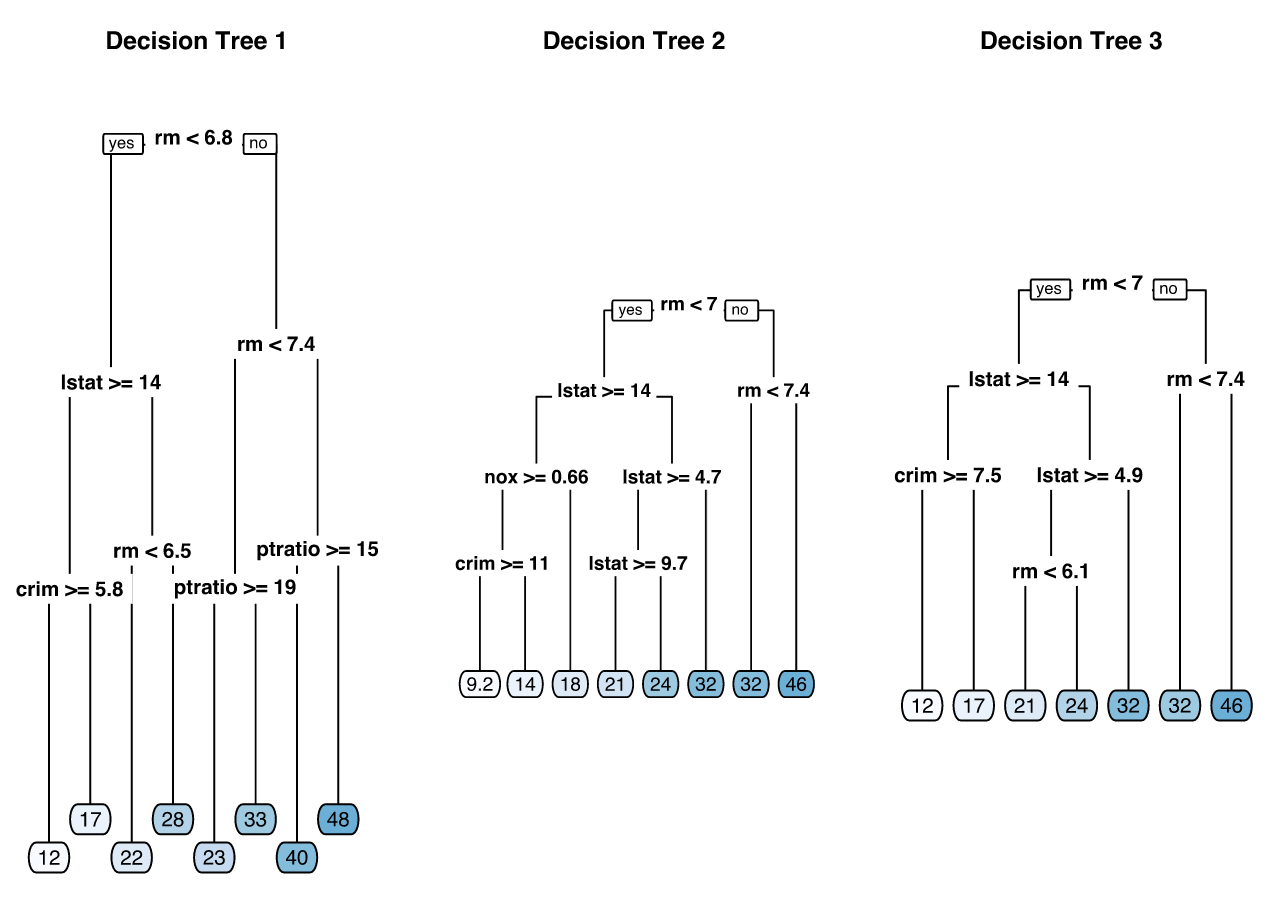
\includegraphics{figure/decissiontree.PNG}

\end{frame}

\begin{frame}[fragile]{Regression Trees - preparation}
\protect\hypertarget{regression-trees---preparation}{}

\begin{Shaded}
\begin{Highlighting}[]
\KeywordTok{library}\NormalTok{(rsample)     }\CommentTok{# data splitting }
\KeywordTok{library}\NormalTok{(dplyr)       }\CommentTok{# data wrangling}
\KeywordTok{library}\NormalTok{(rpart)       }\CommentTok{# performing regression trees}
\KeywordTok{library}\NormalTok{(rpart.plot)  }\CommentTok{# plotting regression trees}
\KeywordTok{library}\NormalTok{(ipred)       }\CommentTok{# bagging}
\KeywordTok{library}\NormalTok{(caret)       }\CommentTok{# bagging}
\end{Highlighting}
\end{Shaded}

\end{frame}

\begin{frame}[fragile]{The Ames Housing data}
\protect\hypertarget{the-ames-housing-data}{}

\begin{itemize}
\tightlist
\item
  Again we use the Ames dataset and split it in a test and training
  dataset
\end{itemize}

\begin{Shaded}
\begin{Highlighting}[]
\KeywordTok{set.seed}\NormalTok{(}\DecValTok{123}\NormalTok{)}
\NormalTok{ames_data <-}\StringTok{ }\NormalTok{AmesHousing}\OperatorTok{::}\KeywordTok{make_ames}\NormalTok{()}
\NormalTok{ames_split <-}\StringTok{ }\KeywordTok{initial_split}\NormalTok{(ames_data,}\DataTypeTok{prop =} \FloatTok{.7}\NormalTok{)}
\NormalTok{ames_train <-}\StringTok{ }\KeywordTok{training}\NormalTok{(ames_split)}
\NormalTok{ames_test  <-}\StringTok{ }\KeywordTok{testing}\NormalTok{(ames_split)}
\end{Highlighting}
\end{Shaded}

\end{frame}

\begin{frame}[fragile]{Fit a regression tree using \texttt{rpart}}
\protect\hypertarget{fit-a-regression-tree-using-rpart}{}

\begin{itemize}
\tightlist
\item
  The fitting process and the visual output of regression trees and
  classification trees are very similar.
\item
  Both use the formula method for expressing the model (similar to
  \texttt{lm}).
\item
  When fitting a regression tree, we need to set
  \texttt{method\ =\ "anova"}.
\item
  By default, \texttt{rpart} will make an intelligent guess based on the
  data type of the response column
\item
  But it's recommened to explictly set the method for reproducibility
  reasons (auto-guesser may change in future).
\end{itemize}

\begin{Shaded}
\begin{Highlighting}[]
\NormalTok{m1 <-}\StringTok{ }\KeywordTok{rpart}\NormalTok{(}\DataTypeTok{formula =}\NormalTok{ Sale_Price }\OperatorTok{~}\StringTok{ }\NormalTok{.,}\DataTypeTok{data =}\NormalTok{ ames_train,}
            \DataTypeTok{method  =} \StringTok{"anova"}\NormalTok{)}
\end{Highlighting}
\end{Shaded}

\end{frame}

\begin{frame}[fragile]{the \texttt{m1} output.}
\protect\hypertarget{the-m1-output.}{}

\begin{Shaded}
\begin{Highlighting}[]
\NormalTok{m1}
\end{Highlighting}
\end{Shaded}

\begin{verbatim}
## n= 2051 
## 
## node), split, n, deviance, yval
##       * denotes terminal node
## 
##  1) root 2051 1.329920e+13 181620.20  
##    2) Overall_Qual=Very_Poor,Poor,Fair,Below_Average,Average,Above_Average,Good 1699 4.001092e+12 156147.10  
##      4) Neighborhood=North_Ames,Old_Town,Edwards,Sawyer,Mitchell,Brookside,Iowa_DOT_and_Rail_Road,South_and_West_of_Iowa_State_University,Meadow_Village,Briardale,Northpark_Villa,Blueste 1000 1.298629e+12 131787.90  
##        8) Overall_Qual=Very_Poor,Poor,Fair,Below_Average 195 1.733699e+11  98238.33 *
##        9) Overall_Qual=Average,Above_Average,Good 805 8.526051e+11 139914.80  
##         18) First_Flr_SF< 1150.5 553 3.023384e+11 129936.80 *
##         19) First_Flr_SF>=1150.5 252 3.743907e+11 161810.90 *
##      5) Neighborhood=College_Creek,Somerset,Northridge_Heights,Gilbert,Northwest_Ames,Sawyer_West,Crawford,Timberland,Northridge,Stone_Brook,Clear_Creek,Bloomington_Heights,Veenker,Green_Hills 699 1.260199e+12 190995.90  
##       10) Gr_Liv_Area< 1477.5 300 2.472611e+11 164045.20 *
##       11) Gr_Liv_Area>=1477.5 399 6.311990e+11 211259.60  
##         22) Total_Bsmt_SF< 1004.5 232 1.640427e+11 192946.30 *
##         23) Total_Bsmt_SF>=1004.5 167 2.812570e+11 236700.80 *
##    3) Overall_Qual=Very_Good,Excellent,Very_Excellent 352 2.874510e+12 304571.10  
##      6) Overall_Qual=Very_Good 254 8.855113e+11 273369.50  
##       12) Gr_Liv_Area< 1959.5 155 3.256677e+11 247662.30 *
##       13) Gr_Liv_Area>=1959.5 99 2.970338e+11 313618.30 *
##      7) Overall_Qual=Excellent,Very_Excellent 98 1.100817e+12 385440.30  
##       14) Gr_Liv_Area< 1990 42 7.880164e+10 325358.30 *
##       15) Gr_Liv_Area>=1990 56 7.566917e+11 430501.80  
##         30) Neighborhood=College_Creek,Edwards,Timberland,Veenker 8 1.153051e+11 281887.50 *
##         31) Neighborhood=Old_Town,Somerset,Northridge_Heights,Northridge,Stone_Brook 48 4.352486e+11 455270.80  
##           62) Total_Bsmt_SF< 1433 12 3.143066e+10 360094.20 *
##           63) Total_Bsmt_SF>=1433 36 2.588806e+11 486996.40 *
\end{verbatim}

\end{frame}

\begin{frame}[fragile]{Steps of the splits (m1) - explained}
\protect\hypertarget{steps-of-the-splits-m1---explained}{}

\begin{itemize}
\tightlist
\item
  E.g., we start with 2051 observations at the root node (very
  beginning) and the first variable we split on (that optimizes a
  reduction in SSE) is \texttt{Overall\_Qual}.
\item
  We see that at the first node all observations with
\end{itemize}

\begin{verbatim}
Overall_Qual=Very_Poor,Poor,Fair,Below_Average,Average,
Above_Average,Good
\end{verbatim}

go to the 2nd branch.

\end{frame}

\begin{frame}[fragile]{The 3rd branch}
\protect\hypertarget{the-3rd-branch}{}

\begin{itemize}
\tightlist
\item
  The number of observations in this branch (1699), their average sales
  price (156147.10) and SSE (4.001092e+12) are listed.
\item
  In the 3rd branch we have 352 observations with
\end{itemize}

\texttt{Overall\_Qual=Very\_Good,Excellent,Very\_Excellent}

\begin{itemize}
\tightlist
\item
  their average sales prices is 304571.10 and the SEE in this region is
  2.874510e+12. 
\end{itemize}

\begin{block}{Visualization with \texttt{rpart.plot}}

\begin{itemize}
\tightlist
\item
  In the default print it will show the percentage of data that fall to
  that node and the average sales price for that branch.
\item
  This tree contains 11 internal nodes resulting in 12 terminal nodes.
\item
  This tree is partitioning on 11 variables to produce its model. 
\end{itemize}

\end{block}

\end{frame}

\begin{frame}[fragile]{The package \texttt{rpart.plot}}
\protect\hypertarget{the-package-rpart.plot}{}

\begin{Shaded}
\begin{Highlighting}[]
\KeywordTok{rpart.plot}\NormalTok{(m1)}
\end{Highlighting}
\end{Shaded}

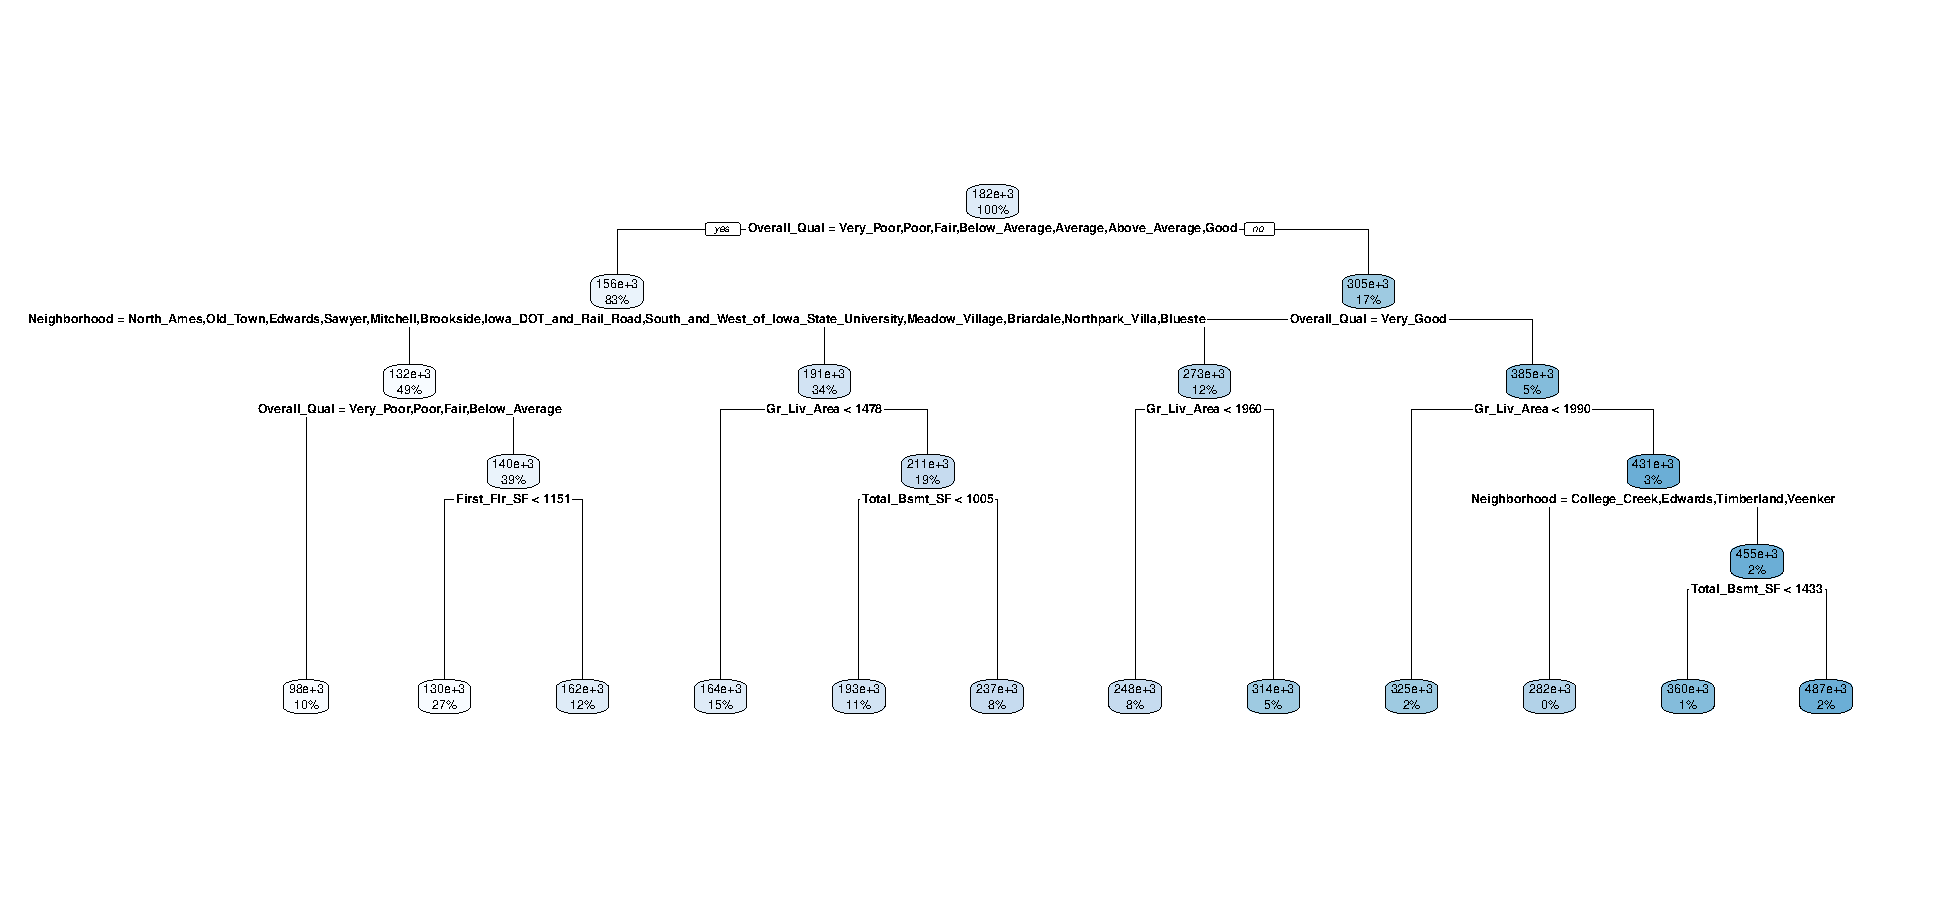
\includegraphics{c1_trees_bagging_files/figure-beamer/unnamed-chunk-7-1.pdf}

\end{frame}

\begin{frame}[fragile]{Behind the scenes}
\protect\hypertarget{behind-the-scenes}{}

There are 80 variables in \texttt{ames\_train}. So what happened?

\begin{itemize}
\tightlist
\item
  There is often a balance to be achieved in the depth and complexity of
  the tree to optimize predictive performance on some unseen data.
\item
  To find this balance, we grow a very large tree as showed and then
  prune it back to find an optimal subtree.
\item
  We find this subtree by using a cost complexity parameter (\(\alpha\))
  that penalizes our objective function for the number of terminal nodes
  of the tree (T).
\end{itemize}

\[
\text{minimize}\{SSE + \alpha|T|\}
\]

\begin{Shaded}
\begin{Highlighting}[]
\NormalTok{TP <-}\StringTok{ }\KeywordTok{prune}\NormalTok{(m1,}\DataTypeTok{cp=}\KeywordTok{median}\NormalTok{(m1}\OperatorTok{$}\NormalTok{cptable[,}\StringTok{'CP'}\NormalTok{]))}
\end{Highlighting}
\end{Shaded}

\end{frame}

\begin{frame}[fragile]{Plot the pruned tree}
\protect\hypertarget{plot-the-pruned-tree}{}

\begin{Shaded}
\begin{Highlighting}[]
\KeywordTok{rpart.plot}\NormalTok{(TP)}
\end{Highlighting}
\end{Shaded}

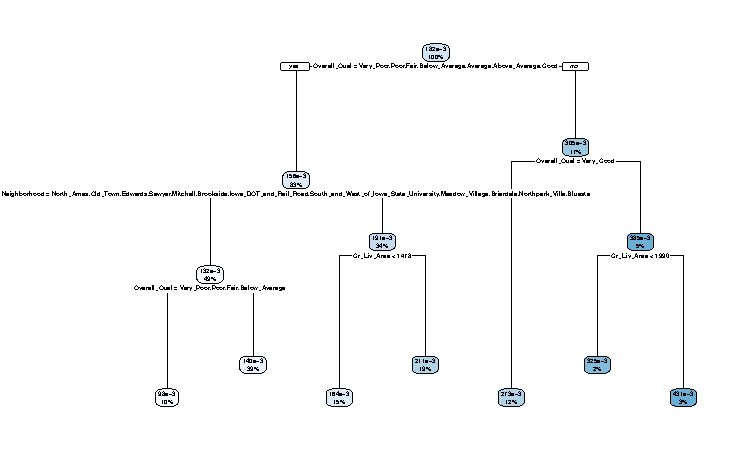
\includegraphics{c1_trees_bagging_files/figure-beamer/unnamed-chunk-9-1.pdf}

\end{frame}

\begin{frame}[fragile]{The \texttt{plotcp}}
\protect\hypertarget{the-plotcp}{}

\begin{itemize}
\tightlist
\item
  Lower x-axis - cost complexity - alpha
\end{itemize}

\begin{Shaded}
\begin{Highlighting}[]
\KeywordTok{plotcp}\NormalTok{(m1)}
\end{Highlighting}
\end{Shaded}

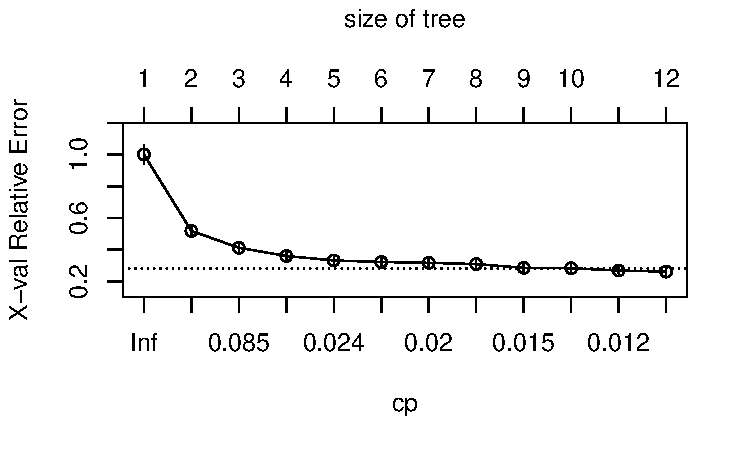
\includegraphics{c1_trees_bagging_files/figure-beamer/unnamed-chunk-10-1.pdf}

\end{frame}

\begin{frame}[fragile]{The 1-SE rule - how many terminal nodes}
\protect\hypertarget{the-1-se-rule---how-many-terminal-nodes}{}

\begin{itemize}
\tightlist
\item
  Breiman et al.~(1984) suggested to use the smallest tree within 1
  standard deviation of the minimum cross validation error (aka the 1-SE
  rule).
\item
  Thus, we could use a tree with 9 terminal nodes and expect to get
  similar results within a small margin of error.
\item
  To illustrate the point of selecting a tree with 12 terminal nodes (or
  9 if you go by the 1-SE rule), we can force \texttt{rpart} to generate
  a full tree by using cp = 0 (no penalty results in a fully grown
  tree).
\end{itemize}

\end{frame}

\begin{frame}[fragile]{Generate a full tree}
\protect\hypertarget{generate-a-full-tree}{}

\begin{itemize}
\tightlist
\item
  After 12 terminal nodes, we see diminishing returns in error reduction
  as the tree grows deeper.
\item
  Thus, we can signifcantly prune our tree and still achieve minimal
  expected error.
\end{itemize}

\begin{Shaded}
\begin{Highlighting}[]
\NormalTok{m2 <-}\StringTok{ }\KeywordTok{rpart}\NormalTok{(}\DataTypeTok{formula =}\NormalTok{ Sale_Price }\OperatorTok{~}\StringTok{ }\NormalTok{.,}\DataTypeTok{data=}\NormalTok{ames_train,}
    \DataTypeTok{method  =} \StringTok{"anova"}\NormalTok{,}\DataTypeTok{control =} \KeywordTok{list}\NormalTok{(}\DataTypeTok{cp =} \DecValTok{0}\NormalTok{, }\DataTypeTok{xval =} \DecValTok{10}\NormalTok{))}
\end{Highlighting}
\end{Shaded}

\begin{itemize}
\tightlist
\item
  \texttt{control} - a list of options that control details of the rpart
  algorithm.
\item
  \texttt{cp} - complexity parameter. Any split that does not decrease
  the overall lack of fit by a factor of cp is not attempted. For
  instance, with anova splitting, this means that the overall R-squared
  must increase by cp at each step (Pruning).
\item
  \texttt{xval} number of cross-validations. 
\end{itemize}

\end{frame}

\begin{frame}[fragile]{Plot the result}
\protect\hypertarget{plot-the-result}{}

\begin{Shaded}
\begin{Highlighting}[]
\KeywordTok{plotcp}\NormalTok{(m2);}\KeywordTok{abline}\NormalTok{(}\DataTypeTok{v =} \DecValTok{12}\NormalTok{, }\DataTypeTok{lty =} \StringTok{"dashed"}\NormalTok{)}
\end{Highlighting}
\end{Shaded}

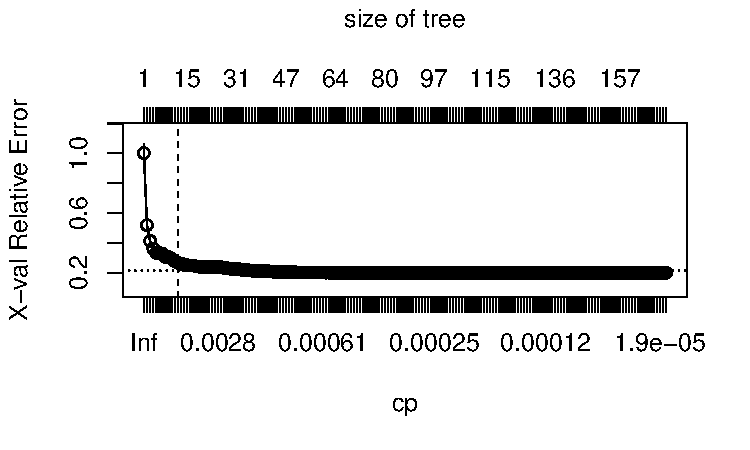
\includegraphics{c1_trees_bagging_files/figure-beamer/unnamed-chunk-12-1.pdf}

\end{frame}

\begin{frame}[fragile]{Automated tuning by default}
\protect\hypertarget{automated-tuning-by-default}{}

\begin{itemize}
\tightlist
\item
  \texttt{rpart} is performing some automated tuning by default, with an
  optimal subtree of 11 splits, 12 terminal nodes, and a cross-validated
  error of 0.272 (note that this error is equivalent to the predicted
  residual error sum of squares statistic
  (\href{https://en.wikipedia.org/wiki/PRESS_statistic}{\textbf{PRESS}})
  but not the MSE).
\item
  We can perform additional tuning to try improve model performance.
\end{itemize}

\end{frame}

\begin{frame}[fragile]{The output \texttt{cptable}}
\protect\hypertarget{the-output-cptable}{}

\begin{Shaded}
\begin{Highlighting}[]
\NormalTok{m1}\OperatorTok{$}\NormalTok{cptable}
\end{Highlighting}
\end{Shaded}

\begin{verbatim}
##            CP nsplit rel error    xerror       xstd
## 1  0.48300624      0 1.0000000 1.0017486 0.05769371
## 2  0.10844747      1 0.5169938 0.5189120 0.02898242
## 3  0.06678458      2 0.4085463 0.4126655 0.02832854
## 4  0.02870391      3 0.3417617 0.3608270 0.02123062
## 5  0.02050153      4 0.3130578 0.3325157 0.02091087
## 6  0.01995037      5 0.2925563 0.3228913 0.02127370
## 7  0.01976132      6 0.2726059 0.3175645 0.02115401
## 8  0.01550003      7 0.2528446 0.3096765 0.02117779
## 9  0.01397824      8 0.2373446 0.2857729 0.01902451
## 10 0.01322455      9 0.2233663 0.2833382 0.01936841
## 11 0.01089820     10 0.2101418 0.2687777 0.01917474
## 12 0.01000000     11 0.1992436 0.2621273 0.01957837
\end{verbatim}

\end{frame}

\begin{frame}[fragile]{Tuning}
\protect\hypertarget{tuning}{}

In addition to the cost complexity (\(\alpha\)) parameter, it is also
common to tune:

\begin{block}{\texttt{minsplit}:}

\begin{itemize}
\tightlist
\item
  The minimum number of data points required to attempt a split before
  it is forced to create a terminal node. The default is 20. Making this
  smaller allows for terminal nodes that may contain only a handful of
  observations to create the predicted value.
\end{itemize}

\end{block}

\begin{block}{\texttt{maxdepth}:}

\begin{itemize}
\tightlist
\item
  The maximum number of internal nodes between the root node and the
  terminal nodes. The default is 30, which is quite liberal and allows
  for fairly large trees to be built.
\end{itemize}

\end{block}

\end{frame}

\begin{frame}[fragile]{Special control argument}
\protect\hypertarget{special-control-argument}{}

\begin{itemize}
\tightlist
\item
  \texttt{rpart} uses a special control argument where we provide a list
  of hyperparameter values.
\item
  E.g., if we want a model with \texttt{minsplit\ =\ 10} and
  \texttt{maxdepth\ =\ 12}, we could execute the following:
\end{itemize}

\begin{Shaded}
\begin{Highlighting}[]
\NormalTok{m3 <-}\StringTok{ }\KeywordTok{rpart}\NormalTok{(}\DataTypeTok{formula =}\NormalTok{ Sale_Price }\OperatorTok{~}\StringTok{ }\NormalTok{.,}\DataTypeTok{data =}\NormalTok{ ames_train,}
    \DataTypeTok{method  =} \StringTok{"anova"}\NormalTok{, }\DataTypeTok{control =} \KeywordTok{list}\NormalTok{(}\DataTypeTok{minsplit =} \DecValTok{10}\NormalTok{, }
                          \DataTypeTok{maxdepth =} \DecValTok{12}\NormalTok{, }\DataTypeTok{xval =} \DecValTok{10}\NormalTok{)}
\NormalTok{)}
\end{Highlighting}
\end{Shaded}

\end{frame}

\begin{frame}[fragile]{The output \texttt{cptable} of model 3}
\protect\hypertarget{the-output-cptable-of-model-3}{}

\begin{Shaded}
\begin{Highlighting}[]
\NormalTok{m3}\OperatorTok{$}\NormalTok{cptable}
\end{Highlighting}
\end{Shaded}

\begin{verbatim}
##            CP nsplit rel error    xerror       xstd
## 1  0.48300624      0 1.0000000 1.0007911 0.05768347
## 2  0.10844747      1 0.5169938 0.5192042 0.02900726
## 3  0.06678458      2 0.4085463 0.4140423 0.02835387
## 4  0.02870391      3 0.3417617 0.3556013 0.02106960
## 5  0.02050153      4 0.3130578 0.3251197 0.02071312
## 6  0.01995037      5 0.2925563 0.3151983 0.02095032
## 7  0.01976132      6 0.2726059 0.3106164 0.02101621
## 8  0.01550003      7 0.2528446 0.2913458 0.01983930
## 9  0.01397824      8 0.2373446 0.2750055 0.01725564
## 10 0.01322455      9 0.2233663 0.2677136 0.01714828
## 11 0.01089820     10 0.2101418 0.2506827 0.01561141
## 12 0.01000000     11 0.1992436 0.2480154 0.01583340
\end{verbatim}

\end{frame}

\begin{frame}[fragile]{Grid search}
\protect\hypertarget{grid-search}{}

\begin{itemize}
\tightlist
\item
  We can avoid it to manually assess multiple models, by performing a
  grid search to automatically search across a range of differently
  tuned models to identify the optimal hyerparameter setting.
\item
  To perform a grid search we first create our hyperparameter grid. 
\end{itemize}

\begin{Shaded}
\begin{Highlighting}[]
\NormalTok{hyper_grid <-}\StringTok{ }\KeywordTok{expand.grid}\NormalTok{(}
  \DataTypeTok{minsplit =} \KeywordTok{seq}\NormalTok{(}\DecValTok{5}\NormalTok{, }\DecValTok{20}\NormalTok{, }\DecValTok{1}\NormalTok{),}
  \DataTypeTok{maxdepth =} \KeywordTok{seq}\NormalTok{(}\DecValTok{8}\NormalTok{, }\DecValTok{15}\NormalTok{, }\DecValTok{1}\NormalTok{)}
\NormalTok{)}
\end{Highlighting}
\end{Shaded}

\begin{itemize}
\tightlist
\item
  The result are 128 combinations - 128 different models.
\end{itemize}

\begin{Shaded}
\begin{Highlighting}[]
\KeywordTok{head}\NormalTok{(hyper_grid)}
\end{Highlighting}
\end{Shaded}

\begin{verbatim}
##   minsplit maxdepth
## 1        5        8
## 2        6        8
## 3        7        8
## 4        8        8
## 5        9        8
## 6       10        8
\end{verbatim}

\begin{Shaded}
\begin{Highlighting}[]
\KeywordTok{nrow}\NormalTok{(hyper_grid)}
\end{Highlighting}
\end{Shaded}

\begin{verbatim}
## [1] 128
\end{verbatim}

\end{frame}

\begin{frame}[fragile]{A loop to autimate modeling}
\protect\hypertarget{a-loop-to-autimate-modeling}{}

\begin{itemize}
\tightlist
\item
  We iterate through each \texttt{minsplit} and \texttt{maxdepth}
  combination.
\item
  We save each model into its own list item.
\end{itemize}

\begin{Shaded}
\begin{Highlighting}[]
\NormalTok{models <-}\StringTok{ }\KeywordTok{list}\NormalTok{()}
\ControlFlowTok{for}\NormalTok{ (i }\ControlFlowTok{in} \DecValTok{1}\OperatorTok{:}\KeywordTok{nrow}\NormalTok{(hyper_grid)) \{}
  \CommentTok{# get minsplit, maxdepth values at row i}
\NormalTok{  minsplit <-}\StringTok{ }\NormalTok{hyper_grid}\OperatorTok{$}\NormalTok{minsplit[i]}
\NormalTok{  maxdepth <-}\StringTok{ }\NormalTok{hyper_grid}\OperatorTok{$}\NormalTok{maxdepth[i]}
  \CommentTok{# train a model and store in the list}
\NormalTok{  models[[i]] <-}\StringTok{ }\KeywordTok{rpart}\NormalTok{(}\DataTypeTok{formula=}\NormalTok{Sale_Price}\OperatorTok{~}\NormalTok{.,}\DataTypeTok{data=}\NormalTok{ames_train,}
    \DataTypeTok{method=}\StringTok{"anova"}\NormalTok{,}\DataTypeTok{control=}\KeywordTok{list}\NormalTok{(}\DataTypeTok{minsplit=}\NormalTok{minsplit,}
                                \DataTypeTok{maxdepth=}\NormalTok{maxdepth)}
\NormalTok{    )}
\NormalTok{\}}
\end{Highlighting}
\end{Shaded}

\end{frame}

\begin{frame}[fragile]{A function to extract the minimum error}
\protect\hypertarget{a-function-to-extract-the-minimum-error}{}

\begin{itemize}
\tightlist
\item
  We create functions to extract the minimum error associated with the
  optimal cost complexity \(\alpha\) value for each model.
\end{itemize}

\begin{Shaded}
\begin{Highlighting}[]
\CommentTok{# function to get optimal cp}
\NormalTok{get_cp <-}\StringTok{ }\ControlFlowTok{function}\NormalTok{(x) \{}
\NormalTok{  min    <-}\StringTok{ }\KeywordTok{which.min}\NormalTok{(x}\OperatorTok{$}\NormalTok{cptable[, }\StringTok{"xerror"}\NormalTok{])}
\NormalTok{  cp <-}\StringTok{ }\NormalTok{x}\OperatorTok{$}\NormalTok{cptable[min, }\StringTok{"CP"}\NormalTok{] }
\NormalTok{\}}

\CommentTok{# function to get minimum error}
\NormalTok{get_min_error <-}\StringTok{ }\ControlFlowTok{function}\NormalTok{(x) \{}
\NormalTok{  min    <-}\StringTok{ }\KeywordTok{which.min}\NormalTok{(x}\OperatorTok{$}\NormalTok{cptable[, }\StringTok{"xerror"}\NormalTok{])}
\NormalTok{  xerror <-}\StringTok{ }\NormalTok{x}\OperatorTok{$}\NormalTok{cptable[min, }\StringTok{"xerror"}\NormalTok{] }
\NormalTok{\}}
\end{Highlighting}
\end{Shaded}

\end{frame}

\begin{frame}[fragile]{Apply the functions}
\protect\hypertarget{apply-the-functions}{}

\begin{Shaded}
\begin{Highlighting}[]
\NormalTok{hyper_grid }\OperatorTok
\StringTok{  }\KeywordTok{mutate}\NormalTok{(}
    \DataTypeTok{cp    =}\NormalTok{ purrr}\OperatorTok{::}\KeywordTok{map_dbl}\NormalTok{(models, get_cp),}
    \DataTypeTok{error =}\NormalTok{ purrr}\OperatorTok{::}\KeywordTok{map_dbl}\NormalTok{(models, get_min_error)}
\NormalTok{    ) }\OperatorTok
\StringTok{  }\KeywordTok{arrange}\NormalTok{(error) }\OperatorTok
\StringTok{  }\KeywordTok{top_n}\NormalTok{(}\OperatorTok{-}\DecValTok{5}\NormalTok{, }\DataTypeTok{wt =}\NormalTok{ error)}
\end{Highlighting}
\end{Shaded}

\begin{verbatim}
##   minsplit maxdepth        cp     error
## 1        5       13 0.0108982 0.2421256
## 2        6        8 0.0100000 0.2453631
## 3       12       10 0.0100000 0.2454067
## 4        8       13 0.0100000 0.2459588
## 5       19        9 0.0100000 0.2460173
\end{verbatim}

\end{frame}

\begin{frame}{Exercise}
\protect\hypertarget{exercise}{}

\begin{block}{Apply the final optimal model}

\end{block}

\begin{block}{Predict on our test dataset}

\end{block}

\end{frame}

\begin{frame}[fragile]{The final optimal model}
\protect\hypertarget{the-final-optimal-model}{}

\begin{block}{Apply the final optimal model:}

\begin{Shaded}
\begin{Highlighting}[]
\NormalTok{optimal_tree <-}\StringTok{ }\KeywordTok{rpart}\NormalTok{(}\DataTypeTok{formula =}\NormalTok{ Sale_Price }\OperatorTok{~}\StringTok{ }\NormalTok{.,}
    \DataTypeTok{data    =}\NormalTok{ ames_train,}\DataTypeTok{method  =} \StringTok{"anova"}\NormalTok{,}
    \DataTypeTok{control =} \KeywordTok{list}\NormalTok{(}\DataTypeTok{minsplit =} \DecValTok{5}\NormalTok{, }\DataTypeTok{maxdepth =} \DecValTok{13}\NormalTok{, }\DataTypeTok{cp =} \FloatTok{0.0108982}\NormalTok{)}
\NormalTok{    )}
\end{Highlighting}
\end{Shaded}

\end{block}

\begin{block}{Predict on our test dataset:}

\begin{Shaded}
\begin{Highlighting}[]
\NormalTok{pred <-}\StringTok{ }\KeywordTok{predict}\NormalTok{(optimal_tree, }\DataTypeTok{newdata =}\NormalTok{ ames_test)}
\end{Highlighting}
\end{Shaded}

\begin{itemize}
\tightlist
\item
  The final RMSE is 39145.39 which suggests that, on average, our
  predicted sales prices are about 39,145 Dollar off from the actual
  sales price.
\end{itemize}

\begin{Shaded}
\begin{Highlighting}[]
\KeywordTok{RMSE}\NormalTok{(}\DataTypeTok{pred =}\NormalTok{ pred, }\DataTypeTok{obs =}\NormalTok{ ames_test}\OperatorTok{$}\NormalTok{Sale_Price)}
\end{Highlighting}
\end{Shaded}

\begin{verbatim}
## [1] 39145.39
\end{verbatim}

\end{block}

\end{frame}

\begin{frame}[fragile]{\href{https://www.r-exercises.com/2016/12/13/recursive-partitioning-and-regression-trees-exercises/}{Exercise:
\texttt{rpart} Kyphosis}}
\protect\hypertarget{exercise-rpart-kyphosis}{}

\begin{block}{Consider the Kyphosis data frame}

\begin{enumerate}
[1)]
\tightlist
\item
  Which variables are in the \texttt{kyphosis} dataset
\item
  Build a tree to classify Kyphosis from Age, Number and Start.
\end{enumerate}

\end{block}

\begin{block}{Consider the tree build above.}

\begin{enumerate}
[1)]
\setcounter{enumi}{2}
\tightlist
\item
  Which variables are used to explain Kyphosis presence?
\item
  How many observations contain the terminal nodes.
\end{enumerate}

\end{block}

\begin{block}{Consider the Kyphosis data frame.}

\begin{enumerate}
[1)]
\setcounter{enumi}{4}
\tightlist
\item
  Build a tree using the first 60 observations of kyphosis.
\item
  Predict the kyphosis presence for the other 21 observations.
\item
  Which is the misclassification rate (prediction error)
\end{enumerate}

\end{block}

\end{frame}

\begin{frame}[fragile]{Exercise: \texttt{rpart} \texttt{iris}}
\protect\hypertarget{exercise-rpart-iris}{}

\begin{block}{Consider the \texttt{iris} data frame}

\begin{enumerate}
[1)]
\tightlist
\item
  Build a tree to classify Species from the other variables.
\item
  Plot the trees, add nodes information.
\end{enumerate}

\end{block}

\begin{block}{Consider the tree build before}

\begin{enumerate}
[1)]
\setcounter{enumi}{2}
\tightlist
\item
  Prune the the using median complexity parameter (cp) associated to the
  tree.
\item
  Plot in the same window, the pruned and the original tree.
\item
  In which terminal nodes is clasified each oobservations of
  \texttt{iris}?
\item
  Which Specie has a flower of \texttt{Petal.Length} greater than 2.45
  and \texttt{Petal.Width} less than 1.75.
\end{enumerate}

\end{block}

\end{frame}

\begin{frame}{Advantages of regression trees}
\protect\hypertarget{advantages-of-regression-trees}{}

\begin{itemize}
\tightlist
\item
  They are very interpretable.
\item
  Making predictions is fast (no complicated calculations, just looking
  up constants in the tree).
\item
  It's easy to understand what variables are important for the
  prediction.
\item
  The internal nodes (splits) are those variables that most largely
  reduced the SSE.
\item
  If some data is missing, we might not be able to go all the way down
  the tree to a leaf, but we can still make a prediction by averaging
  all the leaves in the sub-tree.
\item
  The model provides a non-linear response, so it can work when the true
  regression surface is not smooth.
\item
  If it is smooth, the piecewise-constant surface can approximate it
  arbitrarily closely (with enough leaves).
\item
  There are fast, reliable algorithms to learn these trees.
\end{itemize}

\end{frame}

\begin{frame}{Weaknesses of regression trees}
\protect\hypertarget{weaknesses-of-regression-trees}{}

\begin{itemize}
\tightlist
\item
  Single regression trees have high variance, resulting in unstable
  predictions (an alternative subsample of training data can
  significantly change the terminal nodes).
\item
  Due to the high variance single regression trees have poor predictive
  accuracy.
\end{itemize}

\end{frame}

\begin{frame}{\href{https://elitedatascience.com/overfitting-in-machine-learning}{Ensembling}}
\protect\hypertarget{ensembling}{}

Ensembles are machine learning methods for combining predictions from
multiple separate models.

\begin{block}{Bagging}

attempts to reduce the chance of overfitting complex models.

\begin{itemize}
\tightlist
\item
  It trains a large number of ``strong'' learners in parallel.
\item
  A strong learner is a model that's relatively unconstrained.
\item
  Bagging then combines all the strong learners together in order to
  ``smooth out'' their predictions.
\end{itemize}

\end{block}

\begin{block}{Boosting}

attempts to improve the predictive flexibility of simple models.

\begin{itemize}
\tightlist
\item
  It trains a large number of ``weak'' learners in sequence.
\item
  A weak learner is a constrained model (limit for max depth of tree).
\item
  Each one in the sequence focuses on learning from the mistakes of the
  one before it.
\item
  Boosting combines all the weak learners into a single strong learner.
\end{itemize}

\end{block}

\end{frame}

\begin{frame}{Bagging and boosting}
\protect\hypertarget{bagging-and-boosting}{}

While bagging and boosting are both ensemble methods, they approach the
problem from opposite directions.

Bagging uses complex base models and tries to ``smooth out'' their
predictions, while boosting uses simple base models and tries to
``boost'' their aggregate complexity.

\end{frame}

\begin{frame}{\href{https://www.r-bloggers.com/improve-predictive-performance-in-r-with-bagging/}{Bagging}}
\protect\hypertarget{bagging-1}{}

\begin{itemize}
\tightlist
\item
  Single tree models suffer from high variance, they are highly unstable
  and poor predictors.
\item
  \href{https://en.wikipedia.org/wiki/Decision_tree_pruning}{\textbf{Pruning}}
  helps, but there are alternative methods that exploite the variability
  of single trees in a way that can significantly improve performance.
\item
  Bootstrap aggregating (bagging) is one such approach (originally
  proposed by Breiman, 1996).
\item
  Bagging is a method for combining predictions from different
  regression or classification models.
\item
  The results of the models are then averaged - in the simplest case
  model predictions are included with the same weight.
\item
  The weights could depend on the quality of the model prediction,
  i.e.~``good'' models are more important than ``bad'' models.
\item
  Bagging leads to significantly improved predictions in the case of
  unstable models.
\end{itemize}

\end{frame}

\begin{frame}{Bagging follows three simple steps:}
\protect\hypertarget{bagging-follows-three-simple-steps}{}

\begin{itemize}
\item
  1.) Create \(m\) bootstrap samples from the training data.
  Bootstrapped samples allow us to create many slightly different data
  sets but with the same distribution as the overall training set.
\item
  2.) For each bootstrap sample train a single, unpruned regression
  tree.
\item
  3.) Average individual predictions from each tree to create an overall
  average predicted value.
\end{itemize}

\end{frame}

\begin{frame}{The bagging process.}
\protect\hypertarget{the-bagging-process.}{}

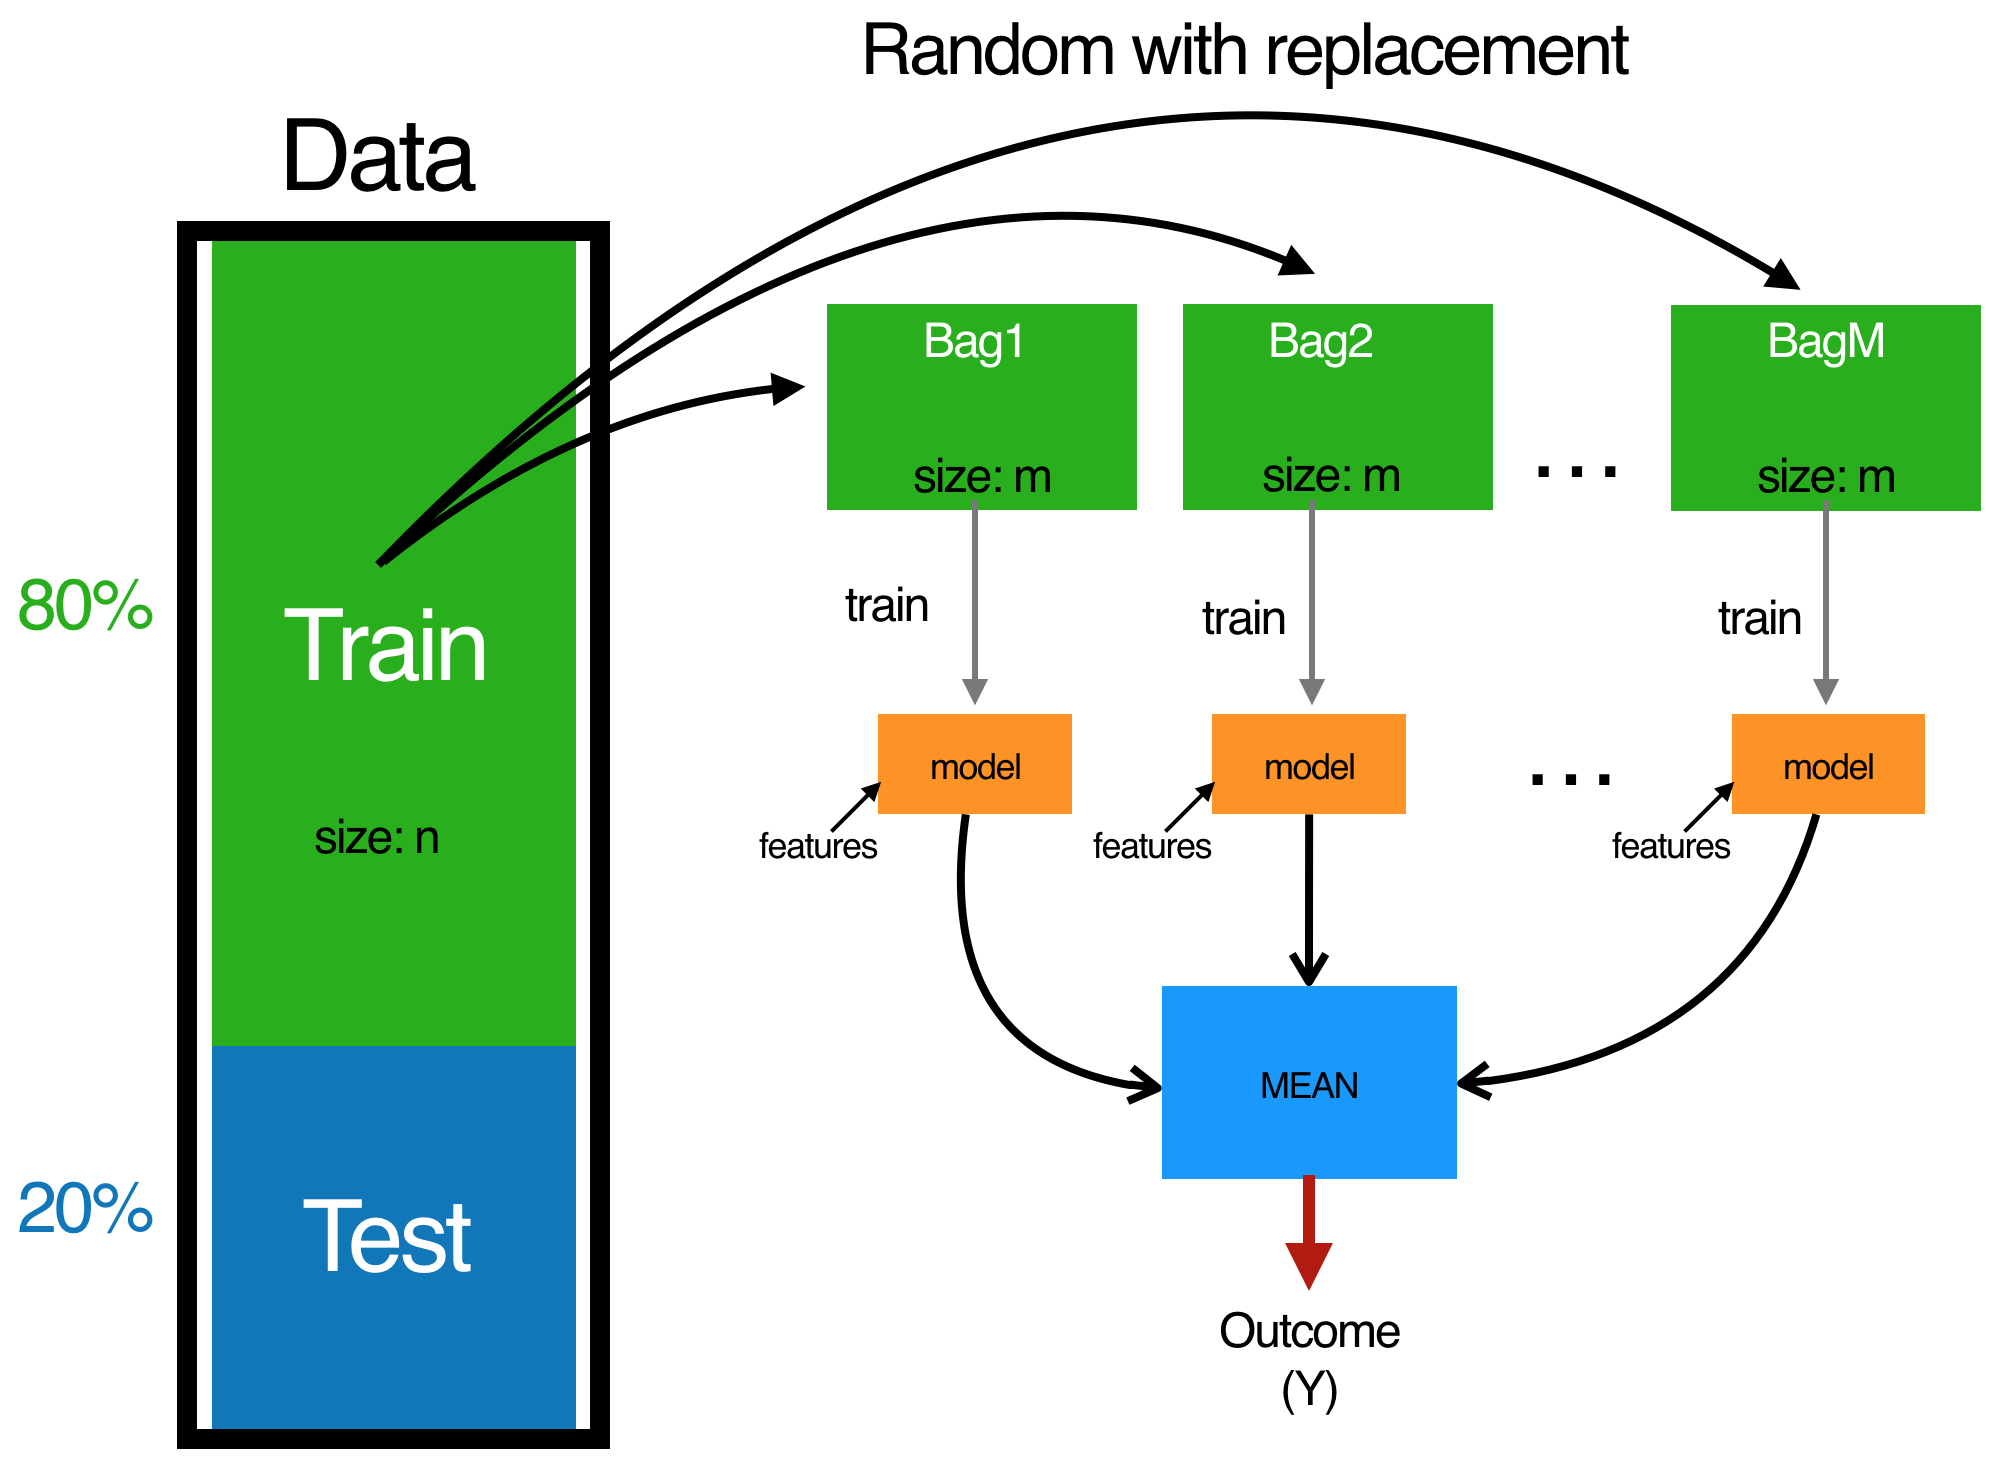
\includegraphics[width=\textwidth,height=0.7\textheight]{figure/bagging3.png}

\end{frame}

\begin{frame}{About bagging}
\protect\hypertarget{about-bagging}{}

\begin{itemize}
\tightlist
\item
  This process can be applied to any regression or classification model;
\item
  It provides the greatest improvement for models that have high
  variance.
\item
  More stable parametric models such as linear regression and
  multi-adaptive regression splines tend to experience less improvement
  in predictive performance.
\item
  On average, a bootstrap sample will contain 63 per cent of the
  training data.
\item
  This leaves about 33 per cent (\(\dfrac{1}{3}\)) of the data out of
  the bootstrapped sample. We call this the out-of-bag (OOB) sample.
\item
  We can use the OOB observations to estimate the model's accuracy,
  creating a natural cross-validation process.
\end{itemize}

\end{frame}

\begin{frame}[fragile]{Bagging with \texttt{ipred}}
\protect\hypertarget{bagging-with-ipred}{}

\begin{itemize}
\tightlist
\item
  Fitting a bagged tree model is quite simple.
\item
  Instead of using \texttt{rpart} we use \texttt{ipred::bagging}.
\item
  We use \texttt{coob\ =\ TRUE} to use the OOB sample to estimate the
  test error.
\end{itemize}

\end{frame}

\begin{frame}[fragile]{Train bagged model}
\protect\hypertarget{train-bagged-model}{}

\begin{Shaded}
\begin{Highlighting}[]
\KeywordTok{set.seed}\NormalTok{(}\DecValTok{123}\NormalTok{)}
\NormalTok{(bagged_m1 <-}\StringTok{ }\KeywordTok{bagging}\NormalTok{(}\DataTypeTok{formula =}\NormalTok{ Sale_Price }\OperatorTok{~}\StringTok{ }\NormalTok{.,}
  \DataTypeTok{data    =}\NormalTok{ ames_train,}\DataTypeTok{coob=} \OtherTok{TRUE}\NormalTok{))}
\end{Highlighting}
\end{Shaded}

\begin{verbatim}
## 
## Bagging regression trees with 25 bootstrap replications 
## 
## Call: bagging.data.frame(formula = Sale_Price ~ ., data = ames_train, 
##     coob = TRUE)
## 
## Out-of-bag estimate of root mean squared error:  36543.37
\end{verbatim}

\begin{itemize}
\tightlist
\item
  We see that our initial estimate error is close to 3000 Dollar less
  than the test error we achieved with our single optimal tree (36543
  vs.~39145)
\end{itemize}

\end{frame}

\begin{frame}{Things to note typically}
\protect\hypertarget{things-to-note-typically}{}

\begin{itemize}
\tightlist
\item
  The more trees the better - we are averaging over more high variance
  single trees.
\item
  We see a dramatic reduction in variance (and hence our error) and
  eventually the reduction in error will flatline 
\item
  You need less than 50 trees to stabilize the error.
\end{itemize}

\end{frame}

\begin{frame}[fragile]{Number of bootstrap samples}
\protect\hypertarget{number-of-bootstrap-samples}{}

\begin{itemize}
\tightlist
\item
  By default bagging performs 25 bootstrap samples and trees but we may
  require more. 
\end{itemize}

\begin{Shaded}
\begin{Highlighting}[]
\CommentTok{# assess 10-50 bagged trees}
\NormalTok{ntree <-}\StringTok{ }\DecValTok{10}\OperatorTok{:}\DecValTok{50} 
\CommentTok{# create empty vector to store OOB RMSE values}
\NormalTok{rmse <-}\StringTok{ }\KeywordTok{vector}\NormalTok{(}\DataTypeTok{mode =} \StringTok{"numeric"}\NormalTok{, }\DataTypeTok{length =} \KeywordTok{length}\NormalTok{(ntree))}
\ControlFlowTok{for}\NormalTok{ (i }\ControlFlowTok{in} \KeywordTok{seq_along}\NormalTok{(ntree)) \{}
  \CommentTok{# reproducibility}
  \KeywordTok{set.seed}\NormalTok{(}\DecValTok{123}\NormalTok{)   }
  \CommentTok{# perform bagged model}
\NormalTok{  model <-}\StringTok{ }\KeywordTok{bagging}\NormalTok{(}\DataTypeTok{formula =}\NormalTok{ Sale_Price }\OperatorTok{~}\StringTok{ }\NormalTok{.,}
  \DataTypeTok{data=}\NormalTok{ames_train,}\DataTypeTok{coob=} \OtherTok{TRUE}\NormalTok{,}\DataTypeTok{nbagg=}\NormalTok{ntree[i]}
\NormalTok{)}
  \CommentTok{# get OOB error}
\NormalTok{  rmse[i] <-}\StringTok{ }\NormalTok{model}\OperatorTok{$}\NormalTok{err   }
\NormalTok{\}}
\end{Highlighting}
\end{Shaded}

\end{frame}

\begin{frame}[fragile]{Plot the result}
\protect\hypertarget{plot-the-result-1}{}

\begin{itemize}
\tightlist
\item
  The error is stabilizing at about 25 trees - we will improve by
  bagging more trees.
\end{itemize}

\begin{Shaded}
\begin{Highlighting}[]
\KeywordTok{plot}\NormalTok{(ntree, rmse, }\DataTypeTok{type =} \StringTok{'l'}\NormalTok{, }\DataTypeTok{lwd =} \DecValTok{2}\NormalTok{)}
\KeywordTok{abline}\NormalTok{(}\DataTypeTok{v =} \DecValTok{25}\NormalTok{, }\DataTypeTok{col =} \StringTok{"red"}\NormalTok{, }\DataTypeTok{lty =} \StringTok{"dashed"}\NormalTok{)}
\end{Highlighting}
\end{Shaded}

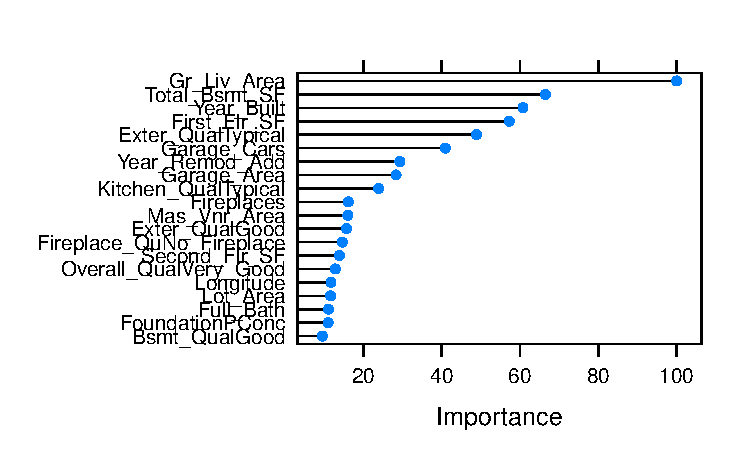
\includegraphics{c1_trees_bagging_files/figure-beamer/unnamed-chunk-26-1.pdf}

\end{frame}

\begin{frame}[fragile]{Bagging with \texttt{caret}}
\protect\hypertarget{bagging-with-caret}{}

\begin{itemize}
\tightlist
\item
  Bagging with \texttt{ipred} is simple but there are some additional
  benefits of bagging with \texttt{caret}.
\end{itemize}

1.) Its easier to perform cross-validation. Although we can use the OOB
error, performing cross validation will provide a more robust
understanding of the true expected test error.

2.) We can assess
\href{https://topepo.github.io/caret/variable-importance.html}{\textbf{variable
importance}} across the bagged trees.

\end{frame}

\begin{frame}[fragile]{\href{https://cran.r-project.org/web/packages/datarobot/vignettes/VariableImportance.html}{Excursus:
Variable importance (vi)}}
\protect\hypertarget{excursus-variable-importance-vi}{}

\begin{itemize}
\tightlist
\item
  vi measures help understand the results obtained from complex machine
  learning models
\item
  There is no general consensus on the ``best'' way to compute - or even
  define - the concept of variable importance.
\item
  See a list of many possible approaches to compute vi in the help file
  of the command \texttt{varImp}
\end{itemize}

\begin{Shaded}
\begin{Highlighting}[]
\NormalTok{?caret}\OperatorTok{::}\NormalTok{varImp}
\end{Highlighting}
\end{Shaded}

\begin{itemize}
\tightlist
\item
  vi refers to how much a given model ``uses'' that variable to make
  accurate predictions. The more a model relies on a variable to make
  predictions, the more important it is for the model.
\end{itemize}

\end{frame}

\begin{frame}[fragile]{A 10-fold cross-validated model.}
\protect\hypertarget{a-10-fold-cross-validated-model.}{}

\begin{Shaded}
\begin{Highlighting}[]
\CommentTok{# Specify 10-fold cross validation}
\NormalTok{ctrl <-}\StringTok{ }\KeywordTok{trainControl}\NormalTok{(}\DataTypeTok{method =} \StringTok{"cv"}\NormalTok{,  }\DataTypeTok{number =} \DecValTok{10}\NormalTok{) }

\NormalTok{bagged_cv <-}\StringTok{ }\KeywordTok{train}\NormalTok{(Sale_Price }\OperatorTok{~}\StringTok{ }\NormalTok{.,}\DataTypeTok{data =}\NormalTok{ ames_train,}
  \DataTypeTok{method =} \StringTok{"treebag"}\NormalTok{,}\DataTypeTok{trControl =}\NormalTok{ ctrl,}\DataTypeTok{importance =} \OtherTok{TRUE}\NormalTok{)}
\end{Highlighting}
\end{Shaded}

\begin{itemize}
\tightlist
\item
  \texttt{treebag}- means we use a bagging tree
\end{itemize}

\end{frame}

\begin{frame}[fragile]{Assess results}
\protect\hypertarget{assess-results}{}

\begin{Shaded}
\begin{Highlighting}[]
\NormalTok{bagged_cv}
\end{Highlighting}
\end{Shaded}

\begin{verbatim}
## Bagged CART 
## 
## 2051 samples
##   80 predictor
## 
## No pre-processing
## Resampling: Cross-Validated (10 fold) 
## Summary of sample sizes: 1846, 1845, 1847, 1845, 1846, 1847, ... 
## Resampling results:
## 
##   RMSE      Rsquared   MAE     
##   36477.25  0.8001783  24059.85
\end{verbatim}

\end{frame}

\begin{frame}[fragile]{Assess results with a plot (top 20 variables)}
\protect\hypertarget{assess-results-with-a-plot-top-20-variables}{}

\begin{itemize}
\tightlist
\item
  Here, variable importance is measured by assessing the total amount
  SSE is decreased by splits over a given predictor, averaged over all
  \(m\) trees.
\end{itemize}

\begin{Shaded}
\begin{Highlighting}[]
\KeywordTok{plot}\NormalTok{(}\KeywordTok{varImp}\NormalTok{(bagged_cv), }\DecValTok{20}\NormalTok{) }
\end{Highlighting}
\end{Shaded}

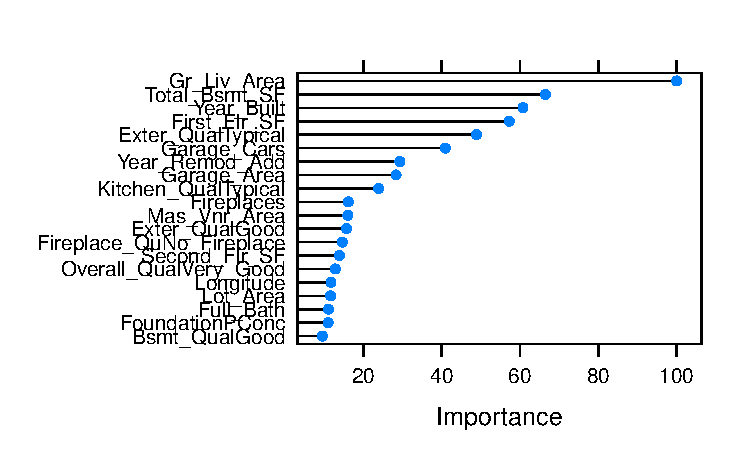
\includegraphics{c1_trees_bagging_files/figure-beamer/unnamed-chunk-30-1.pdf}

\end{frame}

\begin{frame}[fragile]{Extensions}
\protect\hypertarget{extensions}{}

\begin{itemize}
\tightlist
\item
  If we compare this to the test set out of sample we see that our
  cross-validated error estimate was very close.
\end{itemize}

\begin{Shaded}
\begin{Highlighting}[]
\NormalTok{pred <-}\StringTok{ }\KeywordTok{predict}\NormalTok{(bagged_cv, ames_test)}
\KeywordTok{RMSE}\NormalTok{(pred, ames_test}\OperatorTok{$}\NormalTok{Sale_Price)}
\end{Highlighting}
\end{Shaded}

\begin{verbatim}
## [1] 35262.59
\end{verbatim}

\begin{itemize}
\tightlist
\item
  We have successfully reduced our error to about \$35k;
\item
  Extensions of this bagging concept (random forests and GBMs) can
  significantly reduce this further.
\end{itemize}

\end{frame}

\begin{frame}[fragile]{Resources and links}
\protect\hypertarget{resources-and-links}{}

\begin{itemize}
\item
  Breimann (1984) -
  \href{https://www.amazon.com/Classification-Regression-Wadsworth-Statistics-Probability/dp/0412048418}{\textbf{Classification
  and Regression Trees}}
\item
  \href{https://cran.r-project.org/web/packages/partykit/vignettes/ctree.pdf}{\textbf{Vignette}}
  for package \texttt{partykit}
\item
  \href{https://rpubs.com/awanindra01/ctree}{\textbf{Conditional
  Inference Trees}}
\item
  \href{https://stats.stackexchange.com/questions/12140/conditional-inference-trees-vs-traditional-decision-trees}{\textbf{Conditional
  inference trees vs traditional decision trees}}
\item
  \href{https://www.youtube.com/watch?v=6ENTbK3yQUQ}{Video on tree based
  methods}
\item
  \href{https://rstudio-pubs-static.s3.amazonaws.com/64455_df98186f15a64e0ba37177de8b4191fa.html}{An
  example of practical machine learning using R}
\end{itemize}

\end{frame}

\end{document}
